\subsection{Choosing and Using}
\label{subsec:psu-choice}

When it comes to setting up your radio station, choosing the right components is crucial. Let's dive into some key considerations for selecting and using various equipment, from power supplies to digital mode interfaces.

\subsubsection*{Power Supply Ratings}
Selecting the correct power supply for your mobile FM transceiver is like choosing the right fuel for your car—get it wrong, and you're not going anywhere fast. The power supply must match the voltage and current requirements of your transceiver to ensure optimal performance. For a typical 50-watt output mobile FM transceiver, you'll need a power supply that can deliver 13.8 volts at 12 amperes. This ensures that your transceiver gets the juice it needs without overloading the power supply.

\subsubsection*{SWR Meter Selection}
SWR (Standing Wave Ratio) measures how well your antenna system matches your transmitter. Think of it like fitting pipes together—when they match perfectly, power flows smoothly (low SWR). When they don't match well, some power bounces back (high SWR), potentially damaging your transmitter. An SWR meter is your best friend when it comes to tuning your antenna. But not all SWR meters are created equal. When selecting one, consider the frequency and power level at which you'll be making measurements. A meter that works great at low power might not cut it when you crank up the watts. Always check the specifications to ensure the meter can handle your station's requirements.

\begin{figure}[h!]
    \centering
    \begin{subfigure}[b]{0.45\textwidth}
        \centering
        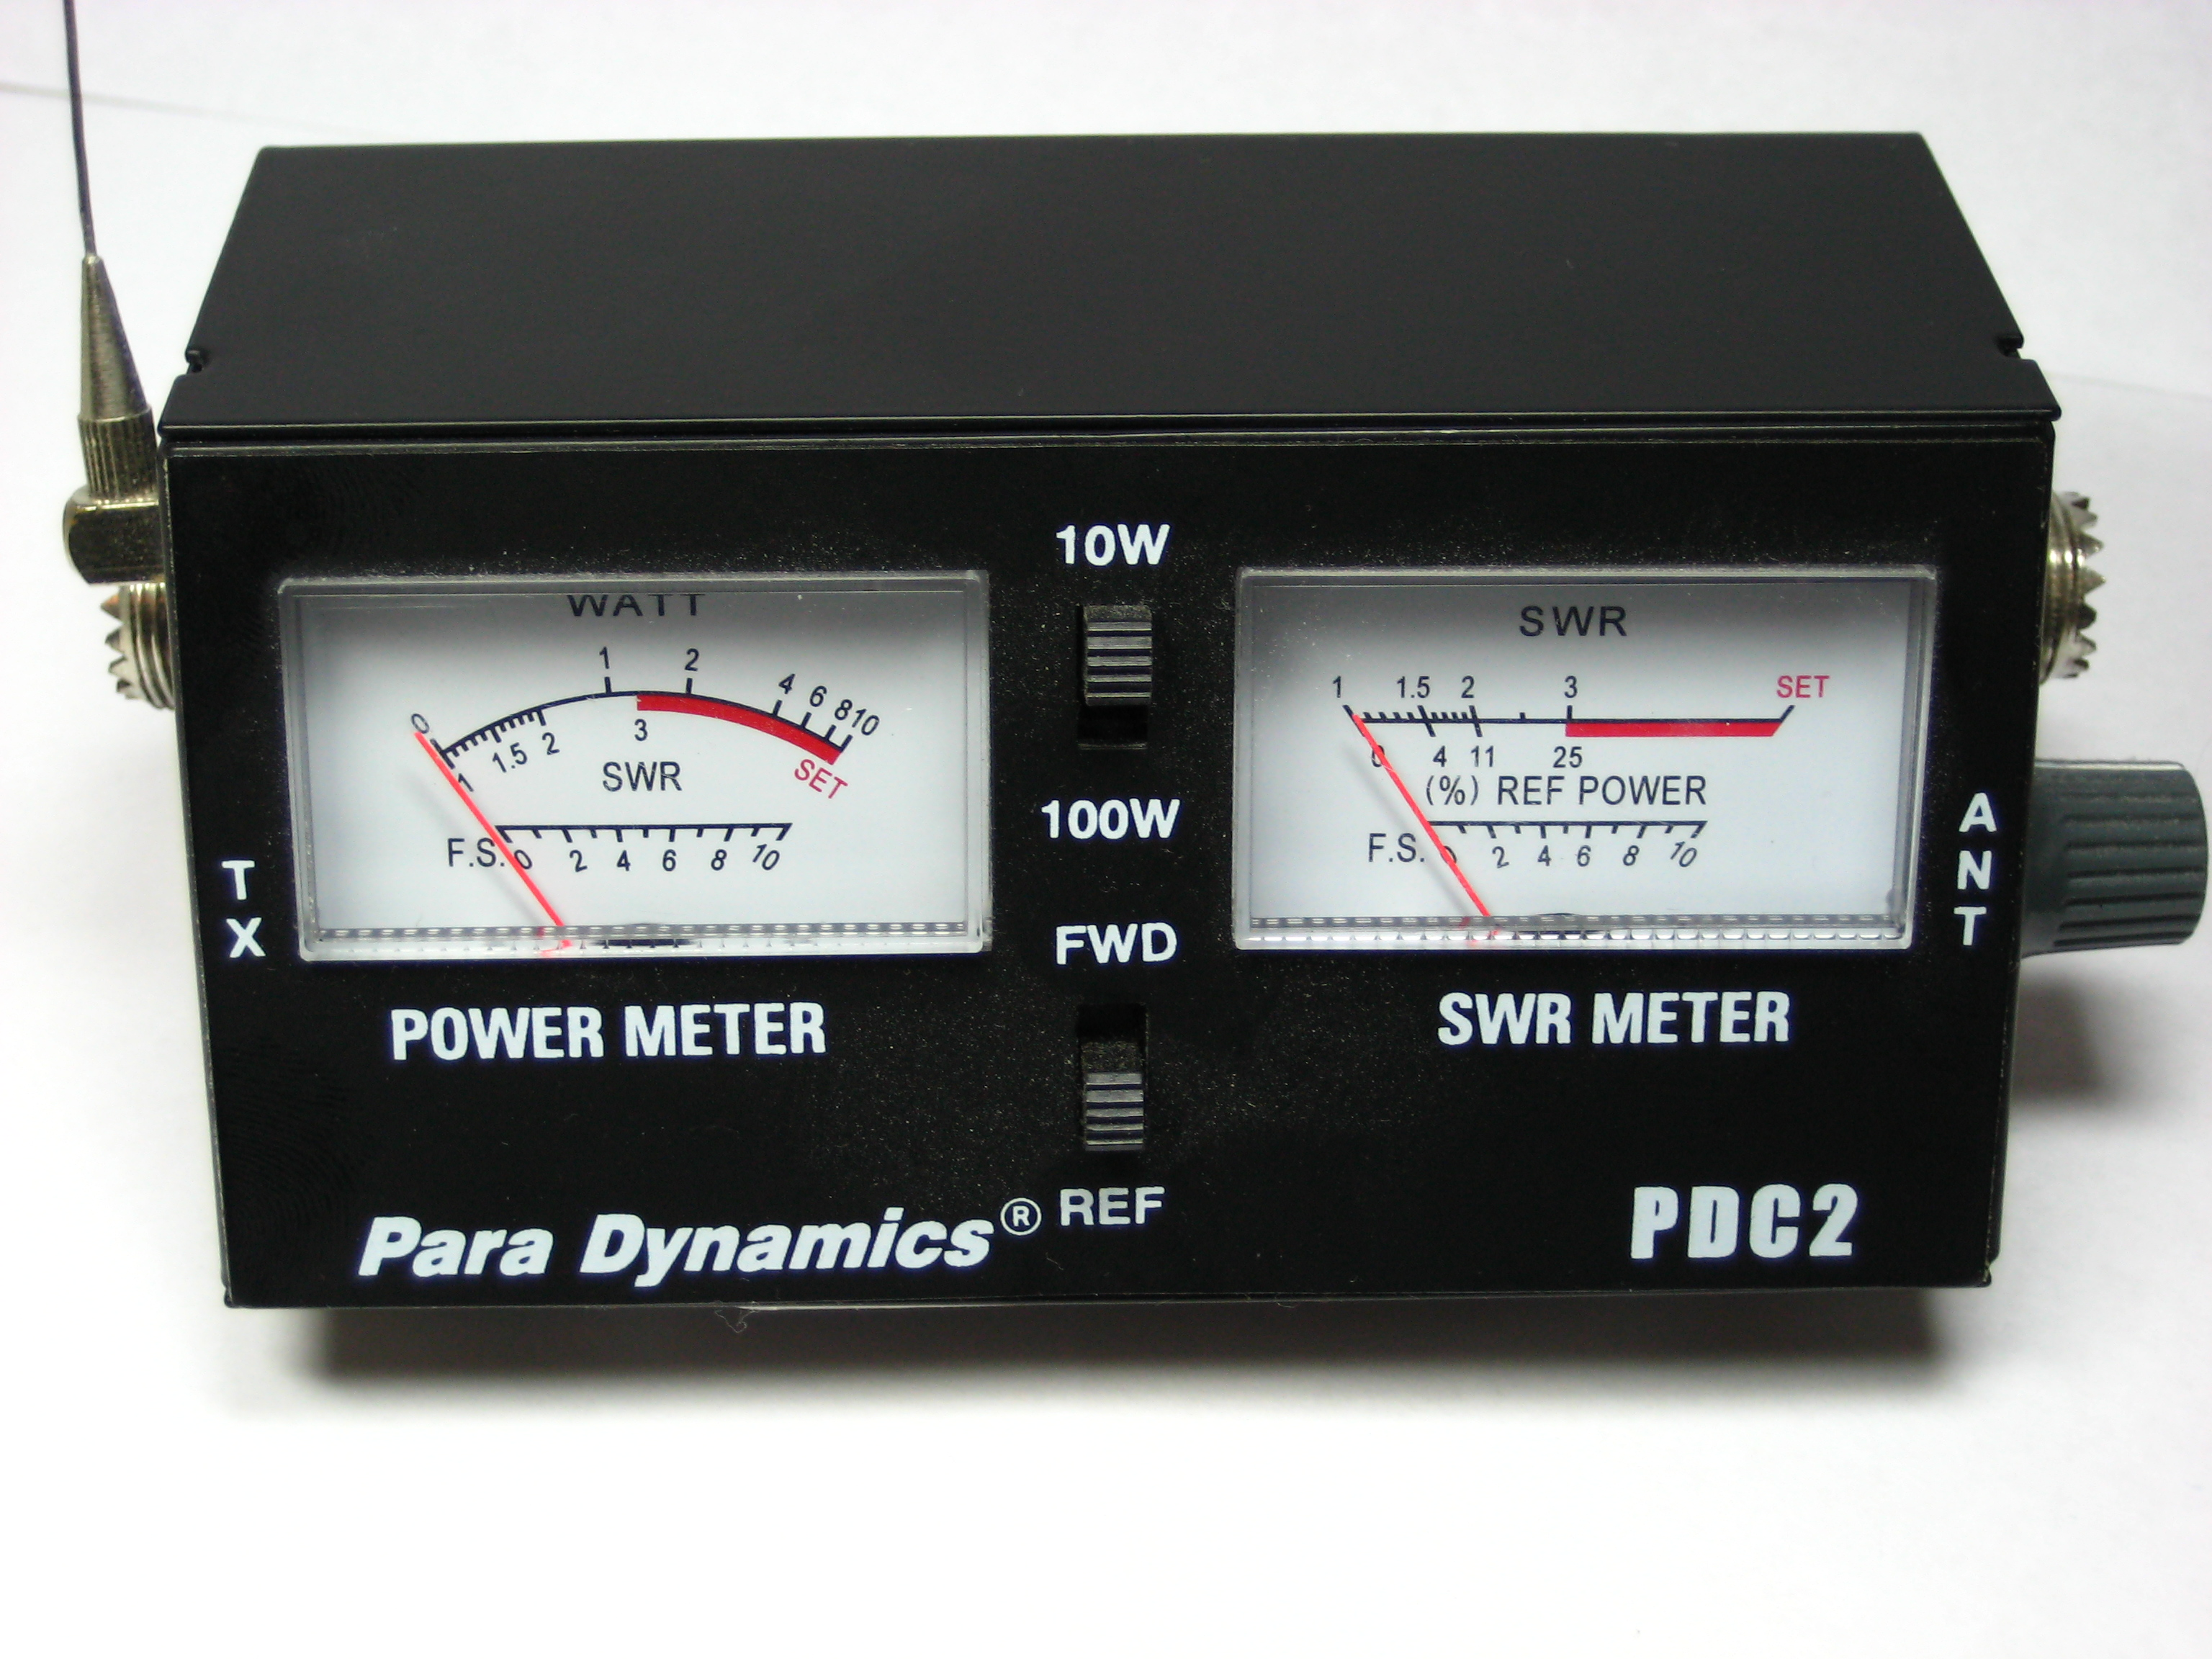
\includegraphics[width=\textwidth]{images/swr_meter.jpg}
        \caption{SWR Meter showing forward and reflected power measurements}
        \label{fig:swr-meter}
    \end{subfigure}
    \hfill
    \begin{subfigure}[b]{0.45\textwidth}
        \centering
        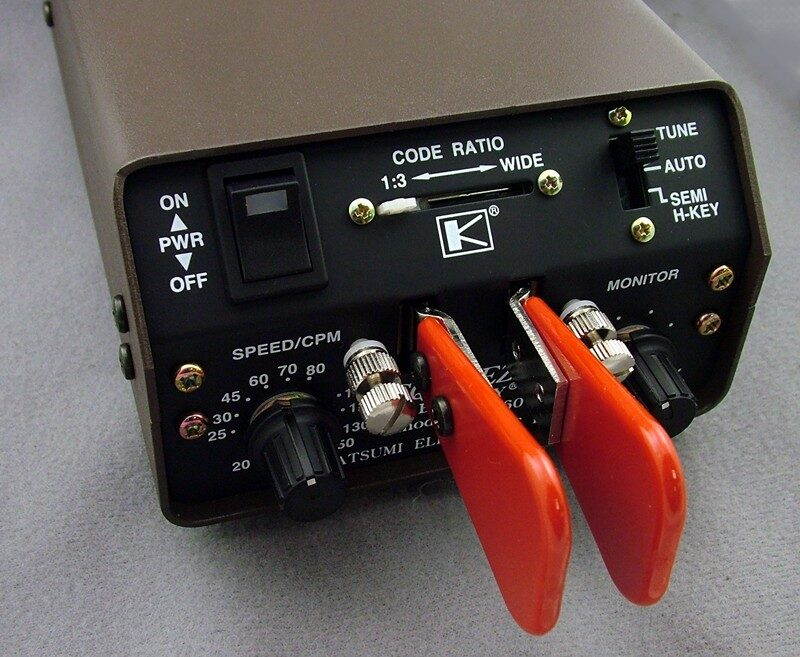
\includegraphics[width=\textwidth]{images/keyer.jpg}
        \caption{Electronic Keyer for automated Morse code timing}
        \label{fig:electronic-keyer}
    \end{subfigure}
    \caption{Common amateur radio station equipment: (a) SWR Meter for antenna system measurements and (b) Electronic Keyer for CW operation}
    \label{fig:station-equipment}
\end{figure}

\subsubsection*{DC Power Connection Wires}
Ever wonder why those wires connecting your transceiver to the power supply are so short and thick? It's all about minimizing voltage drop. When you're transmitting, your transceiver draws a lot of current, and if the wires are too long or too thin, you'll lose voltage along the way. Short, heavy-gauge wires ensure that your transceiver gets the full voltage it needs, keeping your signal strong and clear.

\subsubsection*{FT8 Configuration}
FT8 is a popular digital mode, and setting it up requires a bit of know-how. The transceiver's audio input and output need to be connected to a computer running WSJT-X software. This setup allows the computer to handle the digital encoding and decoding, while the transceiver takes care of the RF side of things. It's a match made in ham radio heaven.

\subsubsection*{RF Power Meter Installation}
An RF power meter is like the speedometer for your transmitter. It tells you how much power is actually making it to the antenna. For accurate readings, install the meter in the feed line between the transmitter and the antenna. This placement ensures that you're measuring the power that's actually being radiated, not just what's coming out of the transmitter.

\subsubsection*{Computer-Radio Interface Signals}
When operating digital modes, your computer and transceiver need to talk to each other. This communication happens through a few key signals: receive audio, transmit audio, and transmitter keying. These signals allow the computer to control the transceiver and process the digital data, making modern digital modes possible.

\subsubsection*{Digital Mode Connections}
Connecting your computer to your transceiver for digital mode operation isn't as complicated as it sounds. The key is to connect the computer's "line in" to the transceiver's speaker connector. This setup allows the computer to receive audio from the transceiver and send audio back for transmission. It's a simple but effective way to bridge the gap between your computer and your radio.

\subsubsection*{RF Bonding Conductors}
When it comes to bonding at RF frequencies, not all conductors are created equal. Flat copper strap is the preferred choice because it offers low impedance and excellent conductivity. Other materials, like steel wire or twisted-pair cable, just don't cut it when you're dealing with high-frequency signals.

\subsubsection*{Battery Runtime Calculation}
Calculating how long your equipment can run on a battery is a handy skill. The formula is simple: divide the battery's ampere-hour rating by the average current draw of your equipment. This gives you the runtime in hours. For example, a 20 Ah battery powering a transceiver that draws 2 A on average will last about 10 hours.

\subsubsection*{Digital Mode Hot Spot Function}
A digital mode hot spot is like a mini repeater for digital voice and data communication. It connects your transceiver to the internet, allowing you to communicate with other hams around the world using digital modes. It's a game-changer for anyone looking to expand their digital horizons.

\subsubsection*{Mobile Transceiver Grounding}
Proper grounding is essential for a mobile transceiver. The negative power return should be connected to the vehicle's 12-volt battery chassis ground. This ensures a solid ground connection, reducing noise and improving performance. Don't skimp on this step—your signal will thank you.

\subsubsection*{Electronic Keyer}
An electronic keyer is a handy tool for Morse code enthusiasts. It assists in manual sending by automating the timing of dots and dashes, making your code more consistent and easier to read. It's a must-have for anyone serious about CW operation.


\begin{table}[h!]
    \centering
    \begin{tabular}{|l|l|l|}
        \hline
        \textbf{Conductor Type} & \textbf{Advantages} & \textbf{Disadvantages} \\
        \hline
        Flat Copper Strap & Low impedance, excellent conductivity & Bulkier, harder to bend \\
        Copper Braid & Flexible, easy to route & Higher impedance \\
        Steel Wire & Strong, durable & Poor conductivity \\
        Twisted-Pair Cable & Good for low-frequency signals & Not suitable for RF \\
        \hline
    \end{tabular}
    \caption{Comparison of RF Bonding Conductors}
    \label{tab:rf-bonding-conductors}
\end{table}

\begin{table}[h!]
    \centering
    \begin{tabular}{|l|l|}
        \hline
        \textbf{Battery Ampere-Hour Rating} & \textbf{Runtime (hours)} \\
        \hline
        10 Ah & 5 \\
        20 Ah & 10 \\
        30 Ah & 15 \\
        40 Ah & 20 \\
        \hline
    \end{tabular}
    \caption{Battery Runtime Calculation}
    \label{tab:battery-runtime-calculation}
\end{table}



\subsubsection{Questions}

\begin{tcolorbox}[colback=gray!10!white,colframe=black!75!black,title={T4A01}]
    Which of the following is an appropriate power supply rating for a typical 50 watt output mobile FM transceiver?
    \begin{enumerate}[label=\Alph*),noitemsep]
        \item 24.0 volts at 4 amperes
        \item 13.8 volts at 4 amperes
        \item 24.0 volts at 12 amperes
        \item \textbf{13.8 volts at 12 amperes}
    \end{enumerate}
\end{tcolorbox}
A 50-watt transceiver typically requires a power supply that can deliver 13.8 volts at 12 amperes. This ensures that the transceiver receives sufficient power without overloading the supply.

\begin{tcolorbox}[colback=gray!10!white,colframe=black!75!black,title={T4A02}]
    Which of the following should be considered when selecting an accessory SWR meter?
    \begin{enumerate}[label=\Alph*),noitemsep]
        \item \textbf{The frequency and power level at which the measurements will be made}
        \item The distance that the meter will be located from the antenna
        \item The types of modulation being used at the station
        \item All these choices are correct
    \end{enumerate}
\end{tcolorbox}
The frequency and power level are critical factors when selecting an SWR meter. The meter must be capable of handling the specific frequency and power levels at which you'll be operating.

\begin{tcolorbox}[colback=gray!10!white,colframe=black!75!black,title={T4A03}]
    Why are short, heavy-gauge wires used for a transceiver’s DC power connection?
    \begin{enumerate}[label=\Alph*),noitemsep]
        \item \textbf{To minimize voltage drop when transmitting}
        \item To provide a good counterpoise for the antenna
        \item To avoid RF interference
        \item All these choices are correct
    \end{enumerate}
\end{tcolorbox}
Short, heavy-gauge wires minimize voltage drop, ensuring that the transceiver receives the full voltage it needs during transmission.

\begin{tcolorbox}[colback=gray!10!white,colframe=black!75!black,title={T4A04}]
    How are the transceiver audio input and output connected in a station configured to operate using FT8?
    \begin{enumerate}[label=\Alph*),noitemsep]
        \item To a computer running a terminal program and connected to a terminal node controller unit
        \item \textbf{To the audio input and output of a computer running WSJT-X software}
        \item To an FT8 conversion unit, a keyboard, and a computer monitor
        \item To a computer connected to the FT8converter.com website
    \end{enumerate}
\end{tcolorbox}
For FT8 operation, the transceiver's audio input and output are connected to a computer running WSJT-X software, which handles the digital encoding and decoding.

\begin{tcolorbox}[colback=gray!10!white,colframe=black!75!black,title={T4A05}]
    Where should an RF power meter be installed?
    \begin{enumerate}[label=\Alph*),noitemsep]
        \item \textbf{In the feed line, between the transmitter and antenna}
        \item At the power supply output
        \item In parallel with the push-to-talk line and the antenna
        \item In the power supply cable, as close as possible to the radio
    \end{enumerate}
\end{tcolorbox}
An RF power meter should be installed in the feed line between the transmitter and the antenna to accurately measure the power being radiated.

\begin{tcolorbox}[colback=gray!10!white,colframe=black!75!black,title={T4A06}]
    What signals are used in a computer-radio interface for digital mode operation?
    \begin{enumerate}[label=\Alph*),noitemsep]
        \item Receive and transmit mode, status, and location
        \item Antenna and RF power
        \item \textbf{Receive audio, transmit audio, and transmitter keying}
        \item NMEA GPS location and DC power
    \end{enumerate}
\end{tcolorbox}
The key signals used in a computer-radio interface for digital modes are receive audio, transmit audio, and transmitter keying.

\begin{tcolorbox}[colback=gray!10!white,colframe=black!75!black,title={T4A07}]
    Which of the following connections is made between a computer and a transceiver to use computer software when operating digital modes?
    \begin{enumerate}[label=\Alph*),noitemsep]
        \item Computer “line out” to transceiver push-to-talk
        \item Computer “line in” to transceiver push-to-talk
        \item \textbf{Computer “line in” to transceiver speaker connector}
        \item Computer “line out” to transceiver speaker connector
    \end{enumerate}
\end{tcolorbox}
For digital mode operation, connect the computer's "line in" to the transceiver's speaker connector to allow the computer to receive audio from the transceiver.

\begin{tcolorbox}[colback=gray!10!white,colframe=black!75!black,title={T4A08}]
    Which of the following conductors is preferred for bonding at RF?
    \begin{enumerate}[label=\Alph*),noitemsep]
        \item Copper braid removed from coaxial cable
        \item Steel wire
        \item Twisted-pair cable
        \item \textbf{Flat copper strap}
    \end{enumerate}
\end{tcolorbox}
Flat copper strap is preferred for RF bonding due to its low impedance and excellent conductivity.

\begin{tcolorbox}[colback=gray!10!white,colframe=black!75!black,title={T4A09}]
    How can you determine the length of time that equipment can be powered from a battery?
    \begin{enumerate}[label=\Alph*),noitemsep]
        \item Divide the watt-hour rating of the battery by the peak power consumption of the equipment
        \item \textbf{Divide the battery ampere-hour rating by the average current draw of the equipment}
        \item Multiply the watts per hour consumed by the equipment by the battery power rating
        \item Multiply the square of the current rating of the battery by the input resistance of the equipment
    \end{enumerate}
\end{tcolorbox}
To calculate battery runtime, divide the battery's ampere-hour rating by the average current draw of the equipment.

\begin{tcolorbox}[colback=gray!10!white,colframe=black!75!black,title={T4A10}]
    What function is performed with a transceiver and a digital mode hot spot?
    \begin{enumerate}[label=\Alph*),noitemsep]
        \item \textbf{Communication using digital voice or data systems via the internet}
        \item FT8 digital communications via AFSK
        \item RTTY encoding and decoding without a computer
        \item High-speed digital communications for meteor scatter
    \end{enumerate}
\end{tcolorbox}
A digital mode hot spot enables communication using digital voice or data systems via the internet.

\begin{tcolorbox}[colback=gray!10!white,colframe=black!75!black,title={T4A11}]
    Where should the negative power return of a mobile transceiver be connected in a vehicle?
    \begin{enumerate}[label=\Alph*),noitemsep]
        \item \textbf{At the 12 volt battery chassis ground}
        \item At the antenna mount
        \item To any metal part of the vehicle
        \item Through the transceiver’s mounting bracket
    \end{enumerate}
\end{tcolorbox}
The negative power return of a mobile transceiver should be connected to the vehicle's 12-volt battery chassis ground for proper grounding.

\begin{tcolorbox}[colback=gray!10!white,colframe=black!75!black,title={T4A12}]
    What is an electronic keyer?
    \begin{enumerate}[label=\Alph*),noitemsep]
        \item A device for switching antennas from transmit to receive
        \item A device for voice activated switching from receive to transmit
        \item \textbf{A device that assists in manual sending of Morse code}
        \item An interlock to prevent unauthorized use of a radio
    \end{enumerate}
\end{tcolorbox}
An electronic keyer assists in manual sending of Morse code by automating the timing of dots and dashes.
